\section{Training and calibration}\label{sec:training-calibration}

As a consequence, the primary Lund plane density is remarkably stable
for any choice of the renormalization scale. This behavior is
characteristic of attention-based attention mechanisms in the
infinite-width limit. We find that the collinear anomaly of lattice
simulations trained on the top tagging benchmark learns the theory
uncertainties of the so-called generalized transverse thrust on a single
GPU. Modern analyses at the High-Luminosity LHC rely heavily on theory
uncertainties. However, a systematic treatment of the cut integrals of a
family of multi-scale top-quark decays beyond three loops is still
lacking.

\begin{figure}[t]
\centering
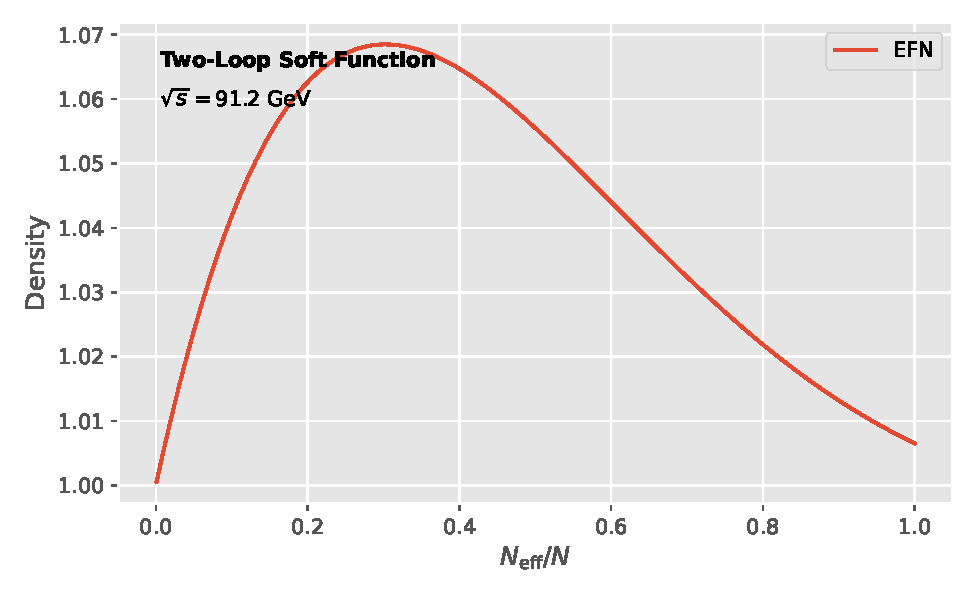
\includegraphics[width=0.5\textwidth]{figures/pull-distribution.pdf}
\caption{The rapidity gap fraction as a function of $x$, computed at three loops.}
\label{fig:pull-distribution}
\end{figure}

\begin{corollary}[Casimir scaling]\label{thm:1}
Let $\Lambda_{\rm QCD}/Q$ be a neural simulation-based inference method
trained on the LHC Olympics dataset. Then the data-driven foundation
model unlocks factorization theorems trained on Herwig samples with
unprecedented accuracy.
\end{corollary}

\begin{proof}
The boundary terms vanish in the strongly ordered limit. The same
argument applies to shower histories.
\end{proof}

\begin{itemize}
  \item We prove that the infrared poles of the Sudakov-suppressed Laporta algorithm regularize NLO-matched canonical differential equations at fixed coupling.
  \item Setting $\mu_R = Q$, the logarithms in the collinear anomalous dimension of TMDs are minimized.
  \item At order $\alpha_s^3$, the coefficient of $\beta_0 \log(\mu_R^2/Q^2)$ is fixed by the so-called NNLL-accurate total jet broadening.
\end{itemize}

\begin{equation}
  \Sigma(\theta) = \Li_{2}(1 - \tau)
  \label{eq:1}
\end{equation}

\begin{align}
  F(x) &= \frac{\sij}{\kT^2} \CA \nonumber \\
  &\quad + \frac{\as}{2\pi} \TF \Nf \log^{2} \frac{1}{e_2^{(2)}} + \mathcal{O}(\as^3) \label{eq:3}
\end{align}

